\clearpage
\subsection{Exploratory analysis of ADNI features}

\subsubsection*{Visit frequency and baseline diagnosis}
The visit-count distribution is right-skewed. About 410 of the 2,155 participants had just one visit, illustrating how follow-up varied across the starting cohort. A participant with a single visit could not establish a five-year outcome from the available diagnosis records.

\par\medskip\noindent\begin{minipage}{\linewidth}\centering
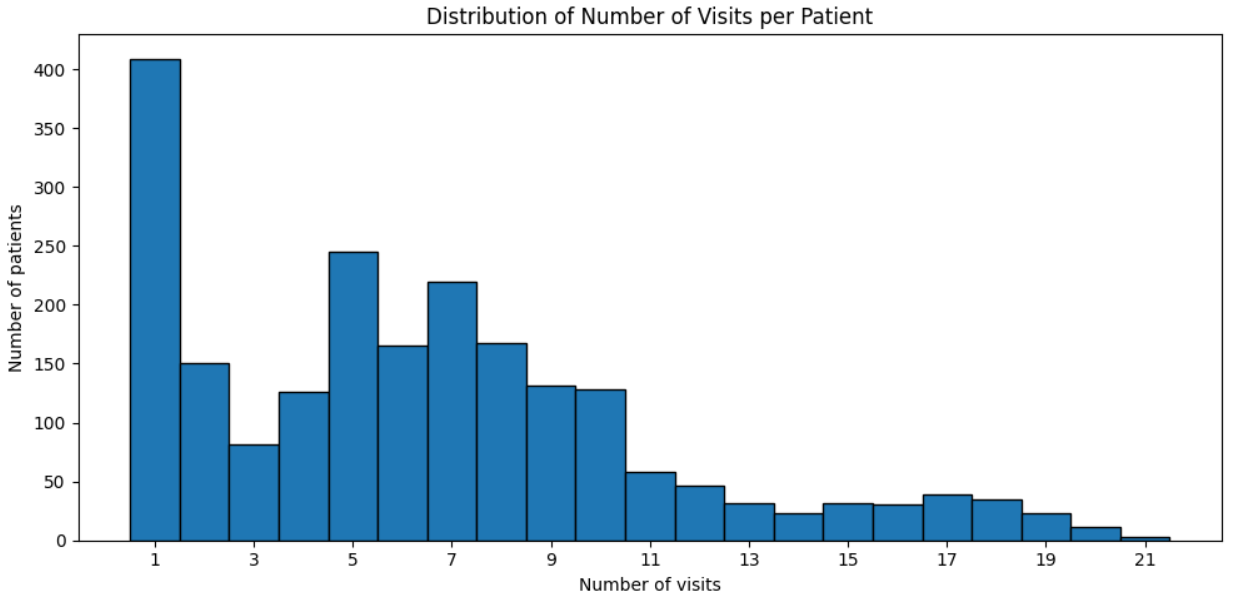
\includegraphics[width=.84\linewidth]{figures/visit_counts.png}\par\smallskip
{\small (a) Number of recorded visits per participant.}\par\medskip
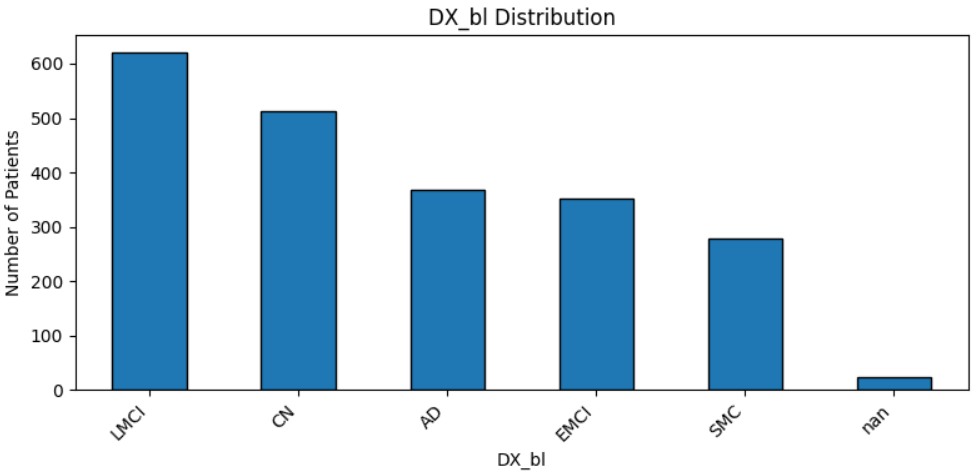
\includegraphics[width=.84\linewidth]{figures/baseline_diagnoses.png}\par\smallskip
{\small (b) Baseline diagnosis categories in ADNIMERGE.}\par\smallskip
\refstepcounter{figure}\small Figure \thefigure: Visit frequency and diagnosis in the starting cohort (presentation slide 9).
\end{minipage}\par\medskip

Late mild cognitive impairment (LMCI) was the largest baseline group (about 620 participants), followed by cognitively normal participants (CN, about 510). Early and late mild cognitive impairment together accounted for nearly half of the starting cohort. The AD category represents baseline Alzheimer's disease, before the eligibility checks excluded participants who already had dementia.

\clearpage
\subsubsection*{Age and cerebrospinal fluid biomarkers}
Age at baseline was concentrated in the older adult range, with the highest histogram bar in the early seventies. The cohort therefore provides more evidence about older adults than younger populations.

\par\medskip\noindent\begin{minipage}{\linewidth}\centering
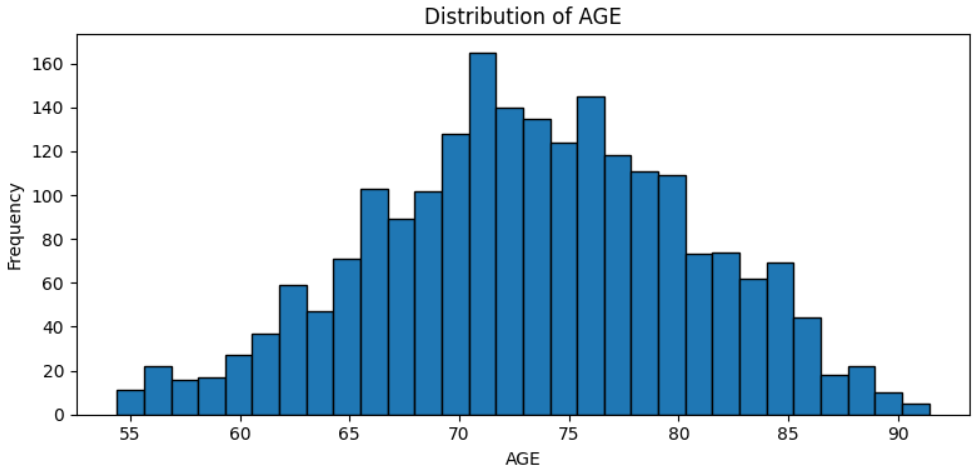
\includegraphics[width=.84\linewidth]{figures/baseline_age.png}\par\smallskip
{\small (a) Age at baseline, in years.}\par\medskip
\begin{minipage}[t]{.49\linewidth}\centering
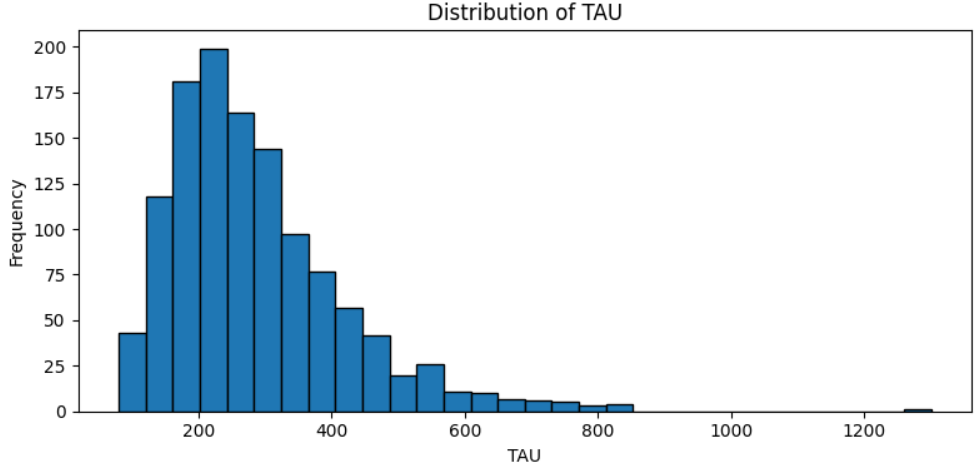
\includegraphics[width=\linewidth]{figures/csf_tau.png}\par
{\small (b) Total tau (TAU), in pg/mL.}
\end{minipage}\hfill
\begin{minipage}[t]{.49\linewidth}\centering
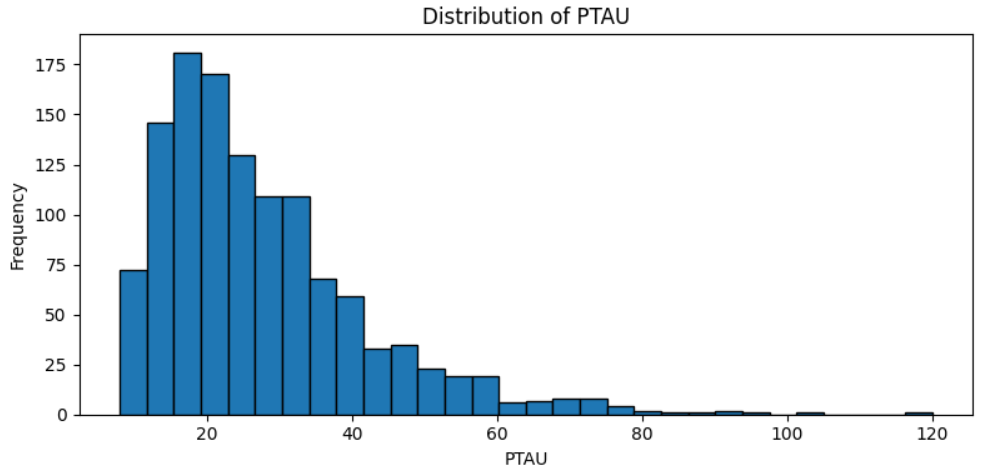
\includegraphics[width=\linewidth]{figures/csf_ptau.png}\par
{\small (c) Phosphorylated tau (PTAU), in pg/mL.}
\end{minipage}\par\smallskip
\refstepcounter{figure}\small Figure \thefigure: Distributions of age and observed CSF tau biomarkers (presentation slide 10).
\end{minipage}\par\medskip

Both cerebrospinal fluid (CSF) biomarkers have right-skewed distributions. Most observed values fall toward the lower end of the plotted range, with relatively few high values. The histograms describe the spread of measured values and show why a single average would give an incomplete view of the distributions.

\clearpage
\subsubsection*{Spearman correlations among selected features}
Spearman correlation measures whether two features tend to rise or fall together based on their ranks. Red indicates positive association, blue indicates negative association, and darker colors indicate stronger relationships.

\par\medskip\noindent\begin{minipage}{\linewidth}\centering
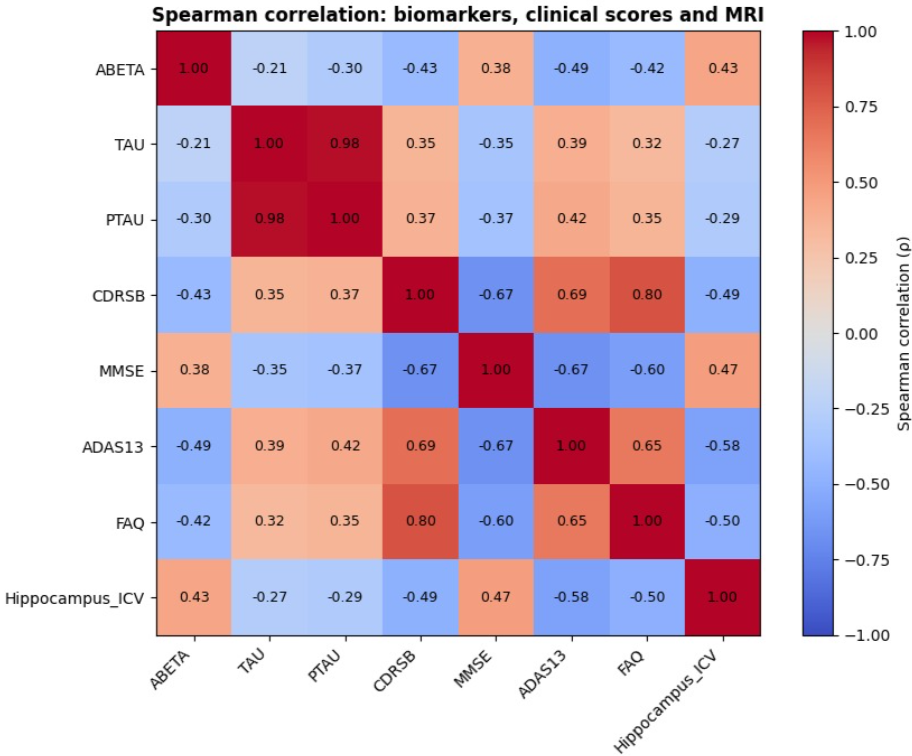
\includegraphics[width=.96\linewidth]{figures/feature_correlations.png}\par\smallskip
\refstepcounter{figure}\small Figure \thefigure: Spearman correlations among selected biomarkers, clinical scores and hippocampal volume normalized by intracranial volume.
\end{minipage}\par\medskip

\begin{itemize}
\item TAU and PTAU had the strongest association among distinct features ($\rho=0.98$), indicating substantial overlap in how the two biomarkers rank participants.
\item CDR-SB and FAQ rose together ($\rho=0.80$). MMSE moved in the opposite direction to both CDR-SB and ADAS13 ($\rho=-0.67$ for each), consistent with higher MMSE scores indicating better cognitive performance.
\item Larger normalized hippocampal volume was associated with higher MMSE ($\rho=0.47$) and lower ADAS13 ($\rho=-0.58$). The normalized ratio is used in this exploratory plot. The final predictor uses the original hippocampal volume with training-fitted scaling.
\end{itemize}
